\documentclass{beamer}
\usepackage[utf8]{inputenc}
\usepackage{xcolor}
\usepackage[T1]{fontenc}
\usepackage[normalem]{ulem}
\usepackage{graphicx}
\usetheme{Antibes}

\definecolor{gray}{rgb}{173,173,173}

\title{Analyse comparée d'arbres taxonomiques}
\author{C. \textsc{Réda}\\supervisée par M \textsc{Nikolski} \& M. \textsc{Raffinot}}
\institute{CGFB, équipe CBIB, Bordeaux}
\date{du 1er juin au 27 juillet 2016}

\begin{document}
\maketitle
\tableofcontents
\setlength{\parindent}{1cm}

\addtobeamertemplate{footline}{\insertframenumber / \inserttotalframenumber}

\section{Déroulement du stage}

%\begin{frame}
%\tableofcontents[currentsection]
%\end{frame}

\subsection{Lieu et modalités du stage}

%\begin{frame}
%\tableofcontents[currentsubsection]
%\end{frame}

\begin{frame}
\frametitle{Informations sur le stage}

\begin{center}

\includegraphics[scale=0.3]{Images/bioinformatique.png}

\begin{itemize}
\item \uline{Lieu :} 
\begin{flushcenter} \bf Centre de Génomique Fonctionnelle \end{flushcenter}
\bigskip
\begin{flushcenter} (CGFB) \end{flushcenter}
\item \uline{Equipe :} 
\begin{flushcenter} \bf Centre de BioInformatique \end{flushcenter}
\bigskip
\begin{flushcenter} (CBIB) \end{flushcenter}
\item \uline{Dates :} 
\begin{flushcenter} du $1^{er}$ juin au 27 juillet 2016 \end{flushcenter}
\end{itemize}

\end{center}

%Une petite équipe d'une dizaine de personnes, informaticiens et biologistes, dans une plateforme de biologie qui propose des prestations et des projets recherche et développement
%lien avec MaBioVis au LaBRI et avec l'hôpital des enfants Pellegrin (à côté) de Bordeaux

\end{frame}

\subsection{Organisation}

%\begin{frame}
%\tableofcontents[currentsubsection]
%\end{frame}

\begin{frame}
\frametitle{Projets de l'équipe CBIB}

\begin{itemize}
\item Une dizaine de logiciels de bioinformatique, dont \alert{Tango};
%TANGO dont le développement est à l'origine du stage
%\pause
\item Participation et $3^{eme}$ place au concours international
\begin{flushcenter}\bf Dream Challenge \end{flushcenter};
%Concours international organisé par le National Cancer Institute (NCI), IBM Research, Sage Bionetworks et la International Society for Computational Biology (ISCB) qui vise à améliorer les logiciels d'analyse des tumeurs.

\begin{center}
\includegraphics[scale=0.1]{Images/dreamchallenge.png}
\end{center}

%\pause
\item Participation au projet
\begin{flushcenter}\bf Galaxy \end{flushcenter};
%Système de fouille et de gestion de données bioinformatique
%\pause
\item Collaborations avec :
     \begin{itemize}
     \item 
      \begin{flushcenter} l'\bf Inra\end{flushcenter} de Bordeaux, 
     %\pause
     \item 
     \begin{flushcenter} le \bf LaBRI\end{flushcenter}, 
     %\pause
     \item  
     \begin{flushcenter} \bf GenoToul Bioinformatique\end{flushcenter} à Toulouse, 
     %\pause
     \item 
     \begin{flushcenter} et l'hôpital \bf Pellegrin\end{flushcenter} à Bordeaux.
     \end{itemize}
\end{itemize}

\end{frame}

\section{Sujet du stage}

%Le stage portait sur les arbres taxonomiques, qui sont des arbres représentant la classification des espèces dans des groupes selon leur histoire évolutive. En métagénomique, qui est l'étude du matériel génétique récupéré dans des environnements naturels, les arbres taxonomiques permettent d'identifier les espèces qui sont présentes dans l'échantillon recueilli, et d'alors déterminer la composition de la population présente dans l'environnement d'où provient l'échantillon.

%La métagénomique est un secteur très actif de nos jours en bioinformatique, grâce à la diminution des prix du traitement de l'ADN (via le séquençage) et au fait qu'elle permet l'étude d'espèces, en particulier de bactéries, non cultivables en laboratoire. Cette discipline a de nombreuses applications en biologie et en médecine.

%Le but de ce stage est d'améliorer l'analyse des données métagénomiques dans un cadre médical. Ici, nous nous concentrons sur l'analyse de l'ADN de bactéries présentes dans l'intestin humain.

%\begin{frame}
%\tableofcontents[currentsection]
%\end{frame}

\subsection{Contexte scientifique}

%\begin{frame}
%\tableofcontents[currentsubsection]
%\end{frame}

\begin{frame}
\frametitle{Traitement du matériel génétique brut}

%récupéré dans l'environnement naturel
\begin{itemize}
\item Extraction de l'ADN par réaction chimique;
%\pause
\item Séquençage de l'ADN obtenu : obtention de la \alert{structure primaire} de l'ADN.
%L'ordre des ensembles de paires de bases construits avec la cytosine, l'adénine, la guanine et la thymine
\end{itemize}
%\pause

\begin{block}{Next-Generation Sequencing (NGS)}
Méthode rapide, relativement bon marché de séquençage de l'ADN, encline aux erreurs. \\
Donne des morceaux de séquences (\alert{reads}) d'une longueur de 32 à 1 000 paires de bases.
\end{block}

\end{frame}

\begin{frame}
\frametitle{Identification des reads à des espèces}

\begin{itemize}
\item Séquençage réalisé sur les gènes 16S;
%Ces gènes contiennent des régions très conservées d'une bactérie à l'autre, et d'autres très variables. Ces dernières permettent d'identifier une bactérie.
%\pause
\bigskip
\item Les limites des \alert{régions hyper variables} sont difficiles à évaluer;
%Ce qui est source d'erreurs dans le séquençage.
%\pause
\bigskip
\item \alert{Alignement} des reads obtenus sur ces régions à des séquences de référence.
%En cas d'alignement optimal (avec une fonction de score maximisée ou minimisée), le read "matche" l'espèce correspondant à la séquence de référence.
%\pause

\begin{center}
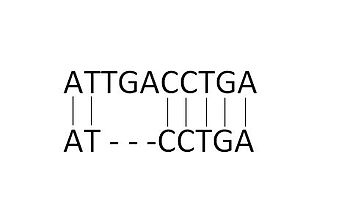
\includegraphics[scale=0.5]{Images/Sequence_gaps.JPG}
\end{center}

\end{itemize}

\end{frame}

\begin{frame}
\frametitle{Arbres taxonomiques}

\begin{block}{Arbre taxonomique} Graphe connexe acyclique non orienté de hauteur bornée, correspondant à l'histoire évolutive du monde vivant.
\end{block}

%Un arbre taxonomique est un arbre enraciné (= graphe connexe acyclique non orienté) de hauteur bornée. Dans la classification du projet GreenGenes, il existe 8 niveaux/générations appelés rangs taxonomiques. Le "premier" niveau correspond au monde vivant, le dernier niveau ne correspond qu'à une seule espèce vivante.

\begin{figure}
\subfigure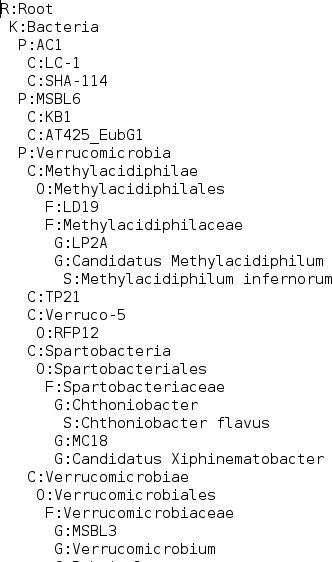
\includegraphics[scale=0.25]{Images/arbretaxo.png}
\subfigure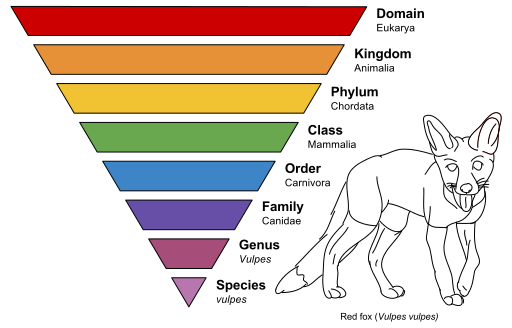
\includegraphics[scale=0.4]{Images/Taxonomic_Rank.png}
\end{figure}

%Il n'existe pas d'arbre taxonomique unique dans la communauté scientifique. Les classifications les plus utilisées sont celles de NCBI, GreenGenes et RDP. La hauteur de ces arbres, ainsi que les rangs taxonomiques, varient d'une base à l'autre.

\end{frame}

\begin{frame}
\frametitle{Arbres taxonomiques}

\begin{block}{Caractéristiques}
\begin{itemize}
\item Plus un noeud est proche de la racine, \\moins son degré est grand;
\item Il y a nettement plus de feuilles que de noeuds internes;
%Pour l'arbre de GreenGenes réduit donné par TANGO, il y a 9 065 noeuds, dont 5 565 feuilles.
\item L'assignation d'un \alert{read} est plus complexe qu'il n'y paraît.
%Un read peut matcher plusieurs séquences de référence, donc plusieurs espèces. Cependant, il ne peut être assigné qu'à une seule espèce. En général, le read est alors assigné au LCA des espèces matchées, qui peut avoir un rang supérieur à S. Mais il existe des algorithmes améliorant cette assignation.
%De plus, il peut exister des erreurs dans le séquençage et donc dans le matching.
\end{itemize}
\end{block}

\end{frame}

\begin{frame}

\begin{alertblock}{Least Common Ancestor (LCA)}
Le LCA de A et B est le dernier noeud de la partie commune des chemins de la racine jusqu'à A et B.
\end{alertblock}

\bigskip

\begin{center}
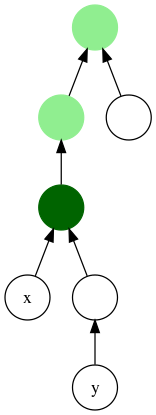
\includegraphics[scale=0.35]{Images/Lowest_common_ancestor.png}
\end{center}

\end{frame}

\begin{frame}
\frametitle{Problématiques de la métagénomique}

Il existe déjà des algorithmes :
%\pause
\begin{itemize}
\item qui améliorent l'alignement des reads aux séquences (Smith et Waterson, 1981);
%\pause
\item qui améliorent l'assignation dans l'arbre des reads matchés (Clemente et al., 2011 : l'outil\textsc{ \bf Tango});
%\pause
\item implémentant des mesures quantifiant la pertinence d'un arbre taxonomique (Robinson et Foulds, 1981)
\item ...
\end{itemize}
%\pause

\begin{center}
Mais...
\end{center}
%Il manque des outils pour comparer les données métagénomiques en fonction d'informations non taxonomiques (ou métadonnées), ou trouver les critères non taxonomiques qui discriminent les échantillons dans un certain ensemble de départ.

%Par exemple, pour des patients atteints de mucovisidose, étant donné des échantillons de leurs flores intestinales, on souhaite savoir si les flores de patients traités par antibiotique sont différentes (et si oui, en quoi) des flores des patients sans traitement.

%Ces questions sont traitées pour le moment par analyse statistique, mais il manque un outil de traitement semi-automatique d'interprétation des données métagénomiques.

\end{frame}

\subsection{Problèmes}

%\begin{frame}
%\tableofcontents[currentsubsection]
%\end{frame}

\begin{frame}
\frametitle{Problème des paires les plus dissemblables}

%Les fichiers d'entrée communs à tous les problèmes étaient l'arbre taxonomique de GreenGenes, une numérotation fixée des échantillons de patients, des bactéries et des métadonnées, et une matrice donnant les valeurs numériques de chaque métadonnée pour chaque échantillon.
\uline{Entrée :} \begin{itemize} \item Une matrice d'occurrence des assignations dans les échantillons. \end{itemize}

\bigskip
\uline{Sortie :} L'ensemble des paires d'échantillons les plus dissemblables.

\end{frame}

\begin{frame}
\frametitle{Problème de compatibilité de la classification}

\uline{Entrée :} \begin{itemize} \item Un sous-ensemble de noeuds/bactéries; \item Un tableau contenant les noeuds matchés dans chaque échantillon; \item Un sous-ensemble de métadonnées. \end{itemize}

\bigskip
\uline{Sortie :} La classification des échantillons selon la valeur des métadonnées du sous-ensemble correspond-elle à la classification des échantillons selon leurs populations bactériennes restreintes au sous-ensemble de noeuds choisis ?

\end{frame}

\begin{frame}
\frametitle{Problème de meilleure classification}

\uline{Entrée :} \begin{itemize} \item Un tableau contenant les noeuds matchés dans chaque échantillon; \item Un sous-ensemble de métadonnées. \end{itemize}

\bigskip
\uline{Sortie :} Un ensemble de noeuds qui donne la meilleure discrimination entre les échantillons par rapport à la classification par rapport aux métadonnées du sous-ensemble.

\end{frame}

\section{Travail de recherche}

%\begin{frame}
%\tableofcontents[currentsection]
%\end{frame}

%A supprimer ?
\subsection{Méthode pseudo-statistique}

%\begin{frame}
%\tableofcontents[currentsubsection]
%\end{frame}

\begin{frame}
\frametitle{Rappel des problèmes}

\begin{itemize}
\item \begin{flushcenter} \bf Problème des paires les plus dissemblables\end{flushcenter}\\ \uline{Sortie :} L'ensemble des paires d'échantillons les plus dissemblables.
\item \uncover<->{ \begin{flushcenter} \bf Problème de compatibilité de la classification\end{flushcenter}\\ \uline{Sortie :} La classification des échantillons selon la valeur des métadonnées du sous-ensemble correspond-elle à la classification des échantillons selon leurs populations bactériennes restreintes au sous-ensemble de noeuds choisis ?}
\item \uncover<->{ \begin{flushcenter} \bf Problème de meilleure classification\end{flushcenter}\\ \uline{Sortie :} Un ensemble de noeuds qui donne la meilleure discrimination entre les échantillons par rapport à la classification par rapport aux métadonnées du sous-ensemble.}
\end{itemize}

%Une méthode qui utilise des mesures sur les populations bactériennes (donc sur les arbres taxonomiques induits par les échantillons), indépendante des métadonnées, pour donner une distance entre les échantillons pour résoudre le problème des paires les plus dissemblables. Cette méthode utilise directement la sortie de TANGO, et donc l'assignation des noeuds dans les échantillons. L'outil associé TAXOTREE peut être considéré comme un outil d'interprétation de TANGO.

\end{frame}

\begin{frame}
\frametitle{Méthode pseudo-statistique : définitions}

\begin{block}{Arbre taxonomique induit par un échantillon}
Forêt de sous-arbres de l'arbre taxonomique de référence constitués des seuls noeuds assignés dans l'échantillon.
\end{block}
%\pause
%*dessin*

\begin{block}{Motif de l'arbre taxonomique (induit)}
Sous-graphe connexe de l'arbre taxonomique (induit).
\end{block}

%*dessin*

\begin{block}{Classes d'échantillons induites par une métadonnée}
Ensemble de groupes d'échantillons disjoints, non vides, selon la valeur numérique -connue- de la métadonnée.
\end{block}

%*exemple*

\end{frame}

\begin{frame}
\frametitle{Mesures utilisées dans \textsc{\bf TaxoTree} (1)}

\begin{block}{Total Ratio}
\begin{center}
$TR(G_{1},G_{2}) = \frac{n}{n_{1} + n_{2} + n}$
\end{center}
\end{block}

%G1, G2 sont deux sous-ensembles d'échantillons
%n est le nombre d'assignations aux noeuds communs aux échantillons de G1 et G2 (noeuds qui sont assignés au moins dans un échantillon de G1 et au moins dans un échantillon de G2)
%ni est le nombre d'assignations aux noeuds assignés seulement dans un échantillon de Gi
%S'intéresse aux populations de noeuds

\begin{figure}
\centering
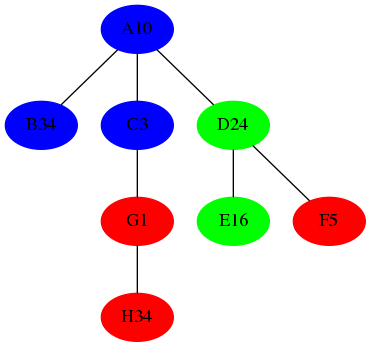
\includegraphics[scale=0.3]{Images/totalratio.png}
\caption{$TR$ = $\frac{10 + 3 + 34}{(1 + 34 + 5) + (10 + 3 + 34) + (24 + 16)} \simeq 0.37$}
\end{figure}

\end{frame}

\begin{frame}
\frametitle{Mesures utilisées dans \textsc{\bf TaxoTree} (2)}

\begin{block}{Pattern Ratio}
\begin{center}
$PR(G_{1},G_{2}) = \frac{n_{common}}{n_{specific}}$
\end{center}
\end{block}

%Un motif commun à deux groupes d'échantillons est un sous-graphe connexe commun aux arbres taxonomiques induits par G1 et G2.

%G1, G2 sont deux sous-ensembles d'échantillons
%n est le nombre d'assignations aux noeuds d'un motif commun (de taille > 1) dans les arbres induits par G1 et G2.
%N est le nombre d'assignations dans les motifs spécifiques à G1 et dans les motifs spécifiques à G2.

\begin{figure}
\centering
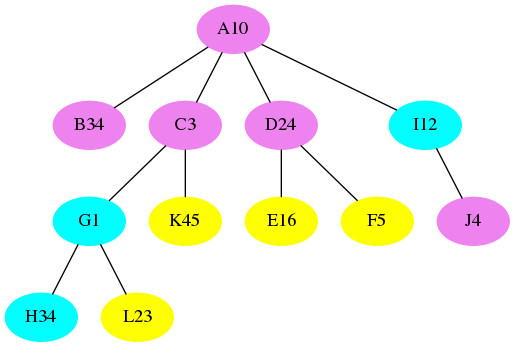
\includegraphics[scale=0.3]{Images/patternratio.png}
\caption{$PR$ = $\frac{10 + 34 + 3 + 24}{(1 + 34 + 12) + (23 + 45 + 16 + 5)} \simeq 0.52$}
\end{figure}

%Se concentre sur la proximité phylogénétique des noeuds des groupes d'échantillons. Cela correspond au "noyau fonctionnel" des bactéries de l'intestin, c'est-à-dire l'ensemble de bactéries nécessaire et suffisant pour faire fonctionner le système digestif.

\end{frame}

\begin{frame}
\frametitle{Mesures utilisées dans \textsc{\bf TaxoTree} (3)}

\begin{block}{Microbial Diversity}
\begin{center}
$MD(G) = \frac{n_{nodes}}{n_{tree}}$
\end{center}
\end{block}

%G est un sous-ensemble d'échantillons
%nnodes est le nombre de noeuds dans l'arbre induit par G
%ntree est le nombre de noeuds dans l'arbre taxonomique complet

\begin{figure}
\centering
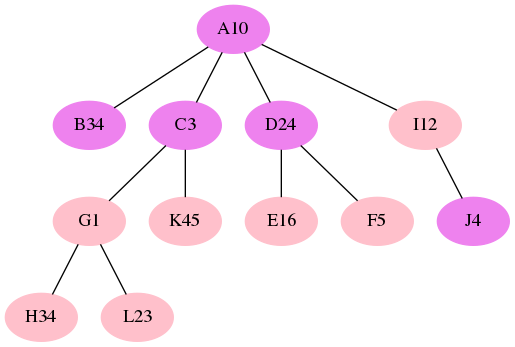
\includegraphics[scale=0.3]{Images/diversity.png}
\caption{$PR$ = $\frac{10 + 34 + 3 + 24}{(1 + 34 + 12) + (23 + 45 + 16 + 5)} \simeq 0.52$}
\end{figure}

%La diversité bactérienne dans l'intestin est le facteur de l'équilibre de cet écosystème fragile.

\end{frame}

\begin{frame}
\frametitle{Distance calculée}

\begin{block}{Coefficient de similarité s}
\begin{itemize}
\item Si $MD(G_{1}) - MD(G_{2}) = 0$ : 
\begin{center}
$ s(G_{1},G_{2}) = TR(G_{1},G_{2}) + PR(G_{1},G_{2})$
\end{center}
\item Sinon : 
\begin{center}
$ s(G_{1},G_{2}) = TR(G_{1},G_{2}) + PR(G_{1},G_{2}) - | MD(G_{1}) - MD(G_{2}) |$
\end{center}
\end{itemize}
\end{block}

\begin{block}{Coefficient de similarité \overline{s}}
\begin{center}
$\overline{s}(G_{1},G_{2}) = \frac{s(G_{1},G_{2}) - E(s)}{\sigma(s)}$
\end{center}
\end{block}

%G1 et G2 sont des sous-ensembles d'échantillons

%Si n est le nombre de classes induites par une métadonnée, on calcule alors s pour chaque paire de classes et on retourne la liste des paires de classes telle que le coefficient de similarité soit inférieur à la valeur du premier quartile.
%On compare alors cette valeur au coefficient de similarité portant sur les valeurs numériques des métadonnées (sommes des coefficients de similarité entre toutes les paires d'échantillons dans des groupes différents, qui sont les sommes des différences en valeur absolue des valeurs de certaines métadonnées -choisies par l'utilisateur)

\uline{Problème :} trouver des mesures pertinentes !

%Caractériser les populations microbiennes sur quelques traits reste grossier, et les phénomènes biologiques mis en jeu ne sont pas connus complètement. Des hypothèses a priori sur ceux-ci sont donc nécessaires, ce qui peut biaiser le résultat final.

\end{frame}

\subsection{Apprentissage supervisé}

%\begin{frame}
%\tableofcontents[currentsubsection]
%\end{frame}

\begin{frame}
\frametitle{Rappel des problèmes}

\begin{itemize}
\item \uncover<->{\begin{flushcenter} \bf Problème des paires les plus dissemblables\end{flushcenter}\\ \uline{Sortie :} L'ensemble des paires d'échantillons les plus dissemblables.}
\item \begin{flushcenter} \bf Problème de compatibilité de la classification\end{flushcenter}\\ \uline{Sortie :} La classification des échantillons selon la valeur des métadonnées du sous-ensemble correspond-elle à la classification des échantillons selon leurs populations bactériennes restreintes au sous-ensemble de noeuds choisis ?
\item \begin{flushcenter} \bf Problème de meilleure classification\end{flushcenter}\\ \uline{Sortie :} Un ensemble de noeuds qui donne la meilleure discrimination entre les échantillons par rapport à la classification par rapport aux métadonnées du sous-ensemble.
\end{itemize}

%Une deuxième approche essaie d'identifier les noeuds de l'arbre taxonomique qui permettent de séparer les échantillons en groupes similaires à ceux obtenus en discriminant les échantillons selon les valeurs numériques de certaines métadonnées, ce qui sous-entend que la présence de ces noeuds est liée à ces métadonnées. Cette approche résout le problème de compatibilité de classification et de meilleure classification. Cette méthode, comme la suivante, néglige l'assignation par TANGO et se concentre sur la sortie de l'alignement des reads avec les séquences de référence, où un read peut être matché à plusieurs séquences de référence. On suppose que l'espèce associée au read est dans l'ensemble des espèces matchées...

\end{frame}

\begin{frame}
\frametitle{Quelques notions de\textsc{ \it Machine Learning }}

\begin{block}{\begin{flushcenter} \it Machine Learning \end{flushcenter}}
Paradigme qui automatise la reconnaissance de certains motifs
\end{block}

%C'est-à-dire que l'ordinateur est capable de trier les données selon leur contenu, sans que le tri soit explicitement programmé. Il permet de traiter de grosses masses de données.

%Utilisé notamment dans la repérage de spams dans les boîtes mail : le programme identifie des mots souvent utilisés dans les emails malveillants ("amour", "bonheur", "fortune") dans les mails de la boîte de réception. Il calcule alors la probabilité que le mail considéré soit non-malveillant sachant qu'il a un telle proportion de ces mots-clés. Si celle-ci est inférieure à celle qu'il soit un spam sachant qu'il a cette proportion de mots-clés, le mail est alors considéré comme un spam. Pour calculer ces probabilités, un ensemble de départ de mails identifiés comme spams et sains est donné au programme pour "l'entraînement". A l'inverse, un programme sans Machine Learning aurait besoin par exemple d'un seuil de fréquences d'apparition des mots-clés (à choisir...) pour pouvoir identifier les spams.

%L'une des plus grandes catégories d'algorithmes de Machine Learning est l'apprentissage supervisé.

%\pause

\begin{block}{Apprentissage supervisé}
Un algorithme d'\alert{apprentissage supervisé} essaie de classer les données dans des catégories \alert{fixées}, en s'aidant d'une connaissance\textsc{ \it a priori } acquise sur un \alert{ensemble d'entraînement}.
\end{block}

%l'exemple des mails. L'un des types de classificateurs les plus utilisés est le classificateur naïf bayésien.

\end{frame}

\begin{frame}
\frametitle{Le classificateur naïf bayésien}

\begin{block}{Classificateur naïf bayésien}
Etant données $k$ classes disjointes de données $(C_{i})_{1 \le i \le k}$, un ensemble de critères $(F_{i})_{1 \le i \le m}$, et une donnée $d$ à classer dans ces classes, ayant $(F_{i} = x_{i})_{1 \le i \le m}$,\\ La classe de $d$ est la classe $C_{j}$ telle que:\\
\begin{center}
$P(C_{j} | F_{1} = x_{1}, ..., F_{m} = x_{m})$\\
$= \max_{h \in \{ 1, ..., k \}}P(C_{h} | F_{1} = x_{1}, ... F_{m} = x_{m})$.\\
\end{center}
\end{block}

%\pause

%Ce classificateur utilise de nombreuses hypothèses a priori pour calculer ces probabilités, comme l'indépendance entre les valeurs numériques des métadonnées.

\end{frame}

\begin{frame}
\frametitle{Calcul de la pertinence de la classification obtenue}

%Ce coefficient calcule la pertinence de la classification pour résoudre le problème de la meilleure classification.

\begin{block}{Coefficient J de Youden}
$J(C) = \frac{TP(C)}{TP(C) + FN(C)} + \frac{TN(C)}{TN(C) + FP(C)} - 1$.
\end{block}

\begin{figure}
\centering
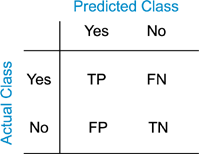
\includegraphics[scale=0.5]{Images/confusionmatrix.png}
\end{figure}

%True Positive TP : données qui appartiennent à C et qui ont été assignées à C par le classificateur
%True Negative TN : données qui n'appartiennent pas à C et qui n'ont pas été assignées à C
%False Negative FN : données qui appartiennent à C et qui n'ont pas été assignées à C
%False Positive FP : données qui n'appartiennt pas à C et qui ont été assignées à C

%Quand $J(C) = 1$, la classification est parfaite; pas de FN et de FP
%Quand $J(C) = 0$, la classification ne fait pas mieux qu'un classificateur aléatoire;
%Quand $J(C) = -1$, la classification est totalement fausse. pas de TN et de TP

%D'après ce qui précède, la meilleure classification est telle que pour chaque classe, le coefficient J de Youden est le plus proche de 1.

\begin{block}{Coefficient \alert{modifié} pour $k$ classes $(C_{i})_{1 \le i \le k}$}
\begin{center}
La quantité $k - \sum{_{i = 1}^{k}}{J(C_{i})}$ est minimale et positive.
\end{center}
\end{block}

\end{frame}

\begin{frame}
\frametitle{Le \textsc{\bf TaxoClassifier} : étapes d'une classification}

Etant donnés un ensemble de métadonnées M (et donc des classes induites par M) et de noeuds N :
%\pause
\bigskip
\begin{enumerate}
\item \alert{Entraînement} du classificateur;
%Choix aléatoire d'un sous-ensemble strict R de l'ensemble des échantillons pour l'entraînement
%Calcul de la probabilité d'avoir un certain noeud de N pour un échantillon
%Comptage et identification des noeuds matchés, appartenant à N, dans chaque échantillon
%\pause
\item Pour chaque échantillon non assigné, calcul des \alert{probabilités postérieures} à chaque classe;
%Les probabilités présentées précédemment
\end{enumerate}
\end{frame}

\begin{frame}
\frametitle{Le classificateur naïf bayésien}
\begin{block}{Classificateur naïf bayésien}
\uncover<->{Etant données $k$ classes disjointes de données $(C_{i})_{1 \le i \le k}$, un ensemble de critères $(F_{i})_{1 \le i \le m}$, et une donnée $d$ à classer dans ces classes, ayant $(F_{i} = x_{i})_{1 \le i \le m}$,\\ La classe de $d$ est la classe $C_{j}$ telle que:\\}
\begin{center}
$P(C_{j} | F_{1} = x_{1}, ..., F_{m} = x_{m})$\\
$= \max_{h \in \{ 1, ..., k \}}P(C_{h} | F_{1} = x_{1}, ... F_{m} = x_{m})$.\\
\end{center}
\end{block}
\end{frame}

\begin{frame}
\frametitle{Le \textsc{\bf TaxoClassifier} : étapes d'une classification}

Etant donnés un ensemble de métadonnées M (et donc des classes induites par M) et de noeuds N :
\bigskip
\begin{enumerate}
\item \alert{Entraînement} du classificateur;
\item Pour chaque échantillon non assigné, calcul des \alert{probabilités postérieures} à chaque classe;
\item Assignation de chaque échantillon à la classe qui maximise la probabilité précédente;
%\pause
\item Retour du coefficient J de Youden \alert{modifié} associé à cette classification.
%\pause
\end{enumerate}

\bigskip

\uline{Problème(s) :} Beaucoup d'hypothèses \textsc{\it a priori}, et de petites améliorations nécessaires pour gérer les cas limites !

\end{frame}

\subsection{Apprentissage non supervisé}

%\begin{frame}
%\tableofcontents[currentsubsection]
%\end{frame}

\begin{frame}
\frametitle{Rappel des problèmes}

\begin{itemize}
\item \uncover<->{ \begin{flushcenter} \bf Problème des paires les plus dissemblables\end{flushcenter}\\ \uline{Sortie :} L'ensemble des paires d'échantillons les plus dissemblables.}
\item \uncover<->{\begin{flushcenter} \bf Problème de compatibilité de la classification\end{flushcenter}\\ \uline{Sortie :} La classification des échantillons selon la valeur des métadonnées du sous-ensemble correspond-elle à la classification des échantillons selon leurs populations bactériennes restreintes au sous-ensemble de noeuds choisis ?}
\item \begin{flushcenter} \bf Problème de meilleure classification\end{flushcenter}\\ \uline{Sortie :} Un ensemble de noeuds qui donne la meilleure discrimination entre les échantillons par rapport à la classification par rapport aux métadonnées du sous-ensemble.

%La troisième méthode, associé à l'outil TaxoCluster, utilise l'apprentissage non supervisé, qui est un autre pan du Machine Learning. Elle consiste à diviser l'ensemble des échantillons en groupes d'échantillons les plus proches, en utilisant une distance ne dépendant que des populations bactériennes matchées, et à comparer les groupes obtenus (des clusters) avec les groupes obtenus en ne considérant que les valeurs numériques des métadonnées. 
\end{itemize}

\end{frame}


%%%%%%%%%%%%%%%%%%%%%%%%%%%%%%%%%%%%%%%%%%%%%%%%ù

\begin{frame}
\frametitle{Clustering}

This section explains what \emph{non-supervised learning} is in \emph{Machine Learning}, and present one of the most common tool in this category, which is the \emph{K-Means algorithm}.

Another broad category in \emph{Machine Learning} is \emph{non-supervised learning}: unlike \emph{supervised learning}, the different classes to which belong the data are not known at first. Provided the set of elements, the algorithm has to distinguish by itself several different classes according to the similarity between the pieces of data from the initial set. This is why one of the most common approach for \emph{non-supervised learning} is \emph{clustering}.

Given a certain distance, \emph{clustering} is the task of gathering objects into disjoint clusters, such that the resulting sets maximize the proximity (in terms of the chosen distance) between elements of a same cluster, and maximize the distance between objects of different clusters.

Although the problem of partitionning $n$ elements into $k$ clusters \cite{PartitionIsNPhard} is \textsc{NP-complete}\cite{NPhard} (see the note in bibliography for a block of \textsc{NP-hardness} and \textsc{NP-completeness}), the \emph{K-Means algorithm} \cite{KMeans} is a rather efficient clustering algorithm. After choosing an integer $k$ that is the estimated number of clusters, the user initializes each cluster with one of the elements of the set. Then, for each non-clustered object, the algorithm computes the distance from this object to the mean of every cluster (in our implementation, it is the sample that minimizes the sum of all distances to the other samples in the same cluster), and assigns the object to the closest cluster. Then it updates the mean of this cluster, and iterates the last two steps until convergence of the solution. For more detailed explanation, see \cite{KMeans}.

Before starting to describe our \textsc{TaxoCluster} method, here are some helpful notations (adapted from \cite{Tango1}):\\

Knowing that $T$ is the whole taxonomic tree, for a certain read $i$, let $M_{i}$ be the set of matched leaves for this read, and $T_{i}$ the subtree of $T$ rooted at the LCA (see above for the block of LCA) of the nodes in $M_{i}$. Let $L_{i}$ be the set of leaves of $T_{i}$, and $N_{i}$ be such as $L_{i} = M_{i} \sqcup N_{i}$ ($M_{i}$ and $N_{i}$ are disjoint, see figure $5.1$).

\begin{figure}[H]
\centering
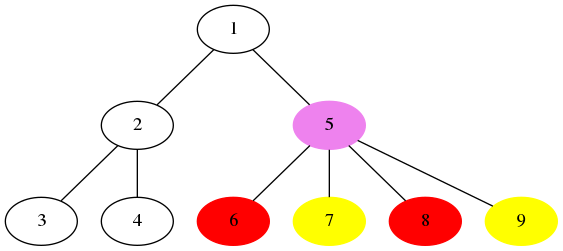
\includegraphics[scale=0.3]{illustrations/timili.png}
\caption{Let T be the whole taxonomic tree. Then for the set of red nodes, the subtree associated is rooted at the violet node, and the total set of leaves for this subtree is the set of yellow and red nodes.}
\end{figure}

Let us define two distances $d_{matched}$ and $d_{consensus}$ over pairs of reads ($R_{i},R_{j}$) for the clustering:
       \begin{itemize} 
       \item \begin{center} $d_{matched}(R_{i},R_{j}) = |M_{i}| + |M_{j}| - 2*|M_{i} \cap M_{j}|$. \end{center}\\ 

It is quite easy to check that $d_{matched}$ is indeed a distance: $d_{matched}$ is symmetric, satisfies the triangle inequality, is non-negative, and $d_{matched}(i,j)$ equals to zero iff $R_{i} = R_{j}$ (The unique relevant equality relation between reads here is the equality between the respective sets of matched nodes, because nobody can know to which node the read should truly be assigned).
       \item Having a fixed parameter $q \in [0,1]$,\\
\begin{center}
$d_{consensus}(R_{i},R_{j}) = |L_{i}| + |L_{j}| - q*(|N_{i}\cap M_{j}| + |N_{j} \cap M_{i}|) - |M_{i} \cap M_{j}|$.\\
\end{center}

It is also easy to check here that $d_{consensus}$ is a distance. This distance corresponds to search a consensus taxonomic tree between the trees induced by the set of nodes matched by the reads \cite{Consensus}.\\

When $q = 0$, we consider a \emph{strict} consensus tree, only keeping leaves matched in both reads.\\
When $q = 1$, we consider a tree having leaves that are matched in at least one of the two reads (see figure $5.2$).

\begin{figure}[H]
\centering
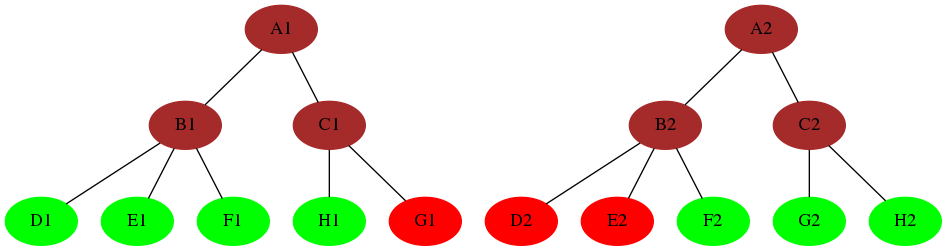
\includegraphics[scale=0.45]{illustrations/distance2.png}
\caption{Let us consider the cyan/blue and orange/red trees (blue and red nodes being the ones matched, the yellow one being matched by the orange tree and not by the blue tree, the two violet nodes are matched in both trees). When $q = 0$, $d_{consensus}(t_{1},t_{2})$ applied to these trees $t_{1}$ and $t_{2}$ is equal to $(2 + 4) - 0 \times (1 + 0) - 2 = 4$. When $q = 1$, $d_{consensus}(t_{1},t_{2})$ is equal to $(2 + 4) - 1 \times (1 + 0) - 2 = 3$}
\end{figure}

       \end{itemize}
\item These distances can easily be extended to samples: if $Reads_{k}$ is the set of reads for sample $S_{k}$,\\
\begin{center}
$d_{consensus}(S_{k},S_{l}) = \sum{r_{k} \in Reads_{k}}{\sum{r_{l} \in Reads_{l}}{d_{consensus}(r_{k},r_{l})}}$.
\end{center} 

Same goes for $d_{matched}$.

\textsc{TaxoCluster} tries to solve problem \textsc{CL.Comp}. It compares trees induced by samples before the assignment of reads, and avoids providing \emph{a priori} hypotheses on the probabilities of being in a certain class of métadonnées values, or of having a certain node. The number $k$ of clusters used in the \textsc{K-Means} algorithm is thus the number of vectors of métadonnées that can be obtained.\\

We use the very same block of classes of métadonnées as in the second method.

\begin{itemize}
\item First the set of samples is clustered into $k$ clusters using $d_{matched}$ distance. 
\item For every cluster, the most remote elements are deleted from the cluster, in order to keep only relevant elements. In our implementation, we discard the points for which sum of all distances to other samples of the same cluster is above the value of the third quartile (of the list of such distances).
\item Then the union of the remaining elements in all clusters is clustered again into $k$ clusters using $d_{consensus}$ distance.
\end{itemize}

The clusters resulting from the second clustering are then compared to the clusters obtained by directly looking at the values of métadonnées in samples. If the two groups of clusters are alike (this is quantified by a special distance), this could mean that there exists a correspondance between the selected métadonnées and the microbial populations. The distance to compare two clusters \textsc{$C_{1}$} and \textsc{$C_{2}$} is d($1$,$2$) $= \frac{|C_{1} \cap C_{2}|}{|C_{1}| + |C_{2}| - |C_{1} \cap C_{2}|} $ (if both clusters are empty, it returns \textsc{None}). The overall distance is (if one of the clusters is empty, then it returns \textsc{None}) $d_{clusters} = \frac{\sum{_{1 \le i < j \le k}}{d(i,j)}}{k}$, where $k$ is the total number of clusters. The program also returns (on demand) the bacteria in common for samples in a same cluster.\\

The whole pipeline has been implemented in \textsc{Python 2.9.7}, and allows to draw and see the clusters in a DOT file.\\

The worst case time complexity is O($n_{samples}^{2} \times (n_{samples} \times n_{paths} \times n_{taxo-nodes} + n_{taxo-nodes}^{2}) \times n_{samples}^{2}$) (see annex for details).\\

(Still in progress) code can be seen at: \\\begin{center}\emph{github.com/kuredatan/taxocluster}.\end{center}

\end{frame}

\begin{frame}
\frametitle{Application au problème de clustering}
\end{frame}

\section{Evaluation des méthodes}

%\begin{frame}
%\tableofcontents[currentsection]
%\end{frame}

\subsection{Implémentation}

%\begin{frame}
%\tableofcontents[currentsubsection]
%\end{frame}

\begin{frame}
\frametitle{Implémentation}
\end{frame}

\subsection{Evaluation}

%\begin{frame}
%\tableofcontents[currentsubsection]
%\end{frame}

\begin{frame}
\frametitle{Evaluation}
\end{frame}

\subsection{Complexité}

%\begin{frame}
%\tableofcontents[currentsubsection]
\end{frame}

\begin{frame}
\frametitle{Complexité}

Theoretically, \textsc{TaxoCluster} is the best method, as it aims at fixing the issues in the first two methods \textsc{TaxoTree} and \textsc{TaxoClassifier}. Indeed, it does not require a special measure on microbial populations, that would induce \emph{a priori} hypotheses on the way these populations should be, with respect to the values of métadonnées. This fact is of paramount importance as most of the biological phenomena still remain partially unknown. Moreover, it does not require strong mathematical hypotheses as it is the case for the \emph{Naive Bayes Classifier}. However, the latter allows more flexibility, whereas it might be irrelevant if the problem is specific enough.\\

Notice that \textsc{TaxoCluster} can only solve the \textsc{Problem of Clustering Compatibility (CL.Comp)}, and not the \textsc{Problem of Best Clustering (CL.BClust)} unlike \textsc{TaxoClassifier}. Furthermore, in terms of worst case time complexity, knowing the actual values for each variable in our test database, it is unfortunately the slowest algorithm:\\

    \begin{table}
      \caption{Complexity for each method: for our test database, $n_{taxo-nodes} = 9,065$, $n_{values} \le 10$, $n_{samples} = 47$ and $n_{paths} = 5,565$}
      \begin{tabular}{|l|c|r|}
        \hline
        \textsc{Method} & \textsc{Theoretical complexity} \\
        \hline
        Statistics & O($n_{taxo-nodes}^{2} \times n_{samples}^{3}$)\\
        \hline
        Supervised learning & O($n_{samples}^{2} \times n_{taxo-nodes}^{2} \times n_{values}$)\\
        \hline
        Non-supervised learning & O($n_{samples}^{2} \times n_{taxo-nodes}\times (n_{samples} \times n_{paths})$)\\
        \hline
      \end{tabular}
    \end{table}

It is worth noticing that nevertheless the three methods can be completely executed on the test computer, even it is just a regular computer (see \textsc{Appendix A}). Nevertheless, to fully validate the results from the algorithms, we should get access to several other databases, and compare them to current biological knowledge and to the output of statistical methods. Due to time limitations, we unfortunately could not use any other database to perform these necessary tests. Moreover, the consistency of results greatly depends on the previous operations applied to input data (have the numeric results been normalized prior to the algorithm? Have all raw material for samples been collected the same way, following a same standard procedure? Has each assignment of read to nodes been performed under the same parameters? and so on). And, last but not least, the final interpretation of the results cannot still be taken into account without the practitionner or a practised biologist's validation.

\end{frame}

\section{Conclusion}

%\begin{frame}
%\tableofcontents[currentsection]
%\end{frame}

\begin{frame}
\frametitle{Bilan et perspectives}

During this internship, we suggested and implemented three methods to analyse data from sequencing according to the métadonnées provided: \textsc{TaxoTree}, \textsc{TaxoClassifier} and \textsc{TaxoCluster}, each of them using a different general paradigm of computer science. We tried to design each method as an improvement of the previous one. These methods solve various clustering-like problems that often occur in biology and medicine. Although their time complexity can probably be improved, the numerical tests done so far appear to be consistent with the medical observations.\\

We also have implemented a class of multi-dimensional lists, and a rather efficient -in regards to the size of our data...- algorithm to reconstruct taxonomic trees from the list of paths from root to every leaf.\\

Use of algorithms from \emph{Machine Learning} in metagenomics is not so new \cite{Nikolski}. However, the last two approaches use a hitherto unseen mix between the common algorithms of \emph{supervised} and \emph{non-supervised learning}, statistics and tree algorithms.\\

On the one hand, a quite large number of comparison problems over labeled unordered trees -taxonomic trees being a special case of this sort of trees- are \textsc{NP-complete}, for instance the problem of tree inclusion \cite{TreeInclusion}. What makes possible efficient algorithms is that the relevant comparison over trees here mainly focuses on the set of leaves for each tree. However, the time complexity of the last two methods, that is \textsc{TaxoClassifier} and \textsc{TaxoCluster}, should still be improved.\\

On the other hand, it would be interesting to test these algorithms on other databases than the one of cystic fibrosis-afflicted patients, so as to see if the resulting correspondances given by the softwares are relevant.\\

The code for all three methods is available on \textsc{GitHub}.\\

\end{frame}

\section{Bibliographie}
\begin{frame}
\frametitle{Sources}

\begin{itemize}
\item \begin{flushleft} \bf Flexible taxonomic assignment of ambiguous sequencing\end{flushcenter}, J. Clemente, J. Jansson et G. Valiente, \begin{flushleft} \it BMC Bioinformatics\end{flushleft}, 2011.
\item \begin{flushleft} \bf Impact de l'antibiothérapie sur le microbiote intestinal chez l'enfant atteint de mucovisidose\end{flushcenter}, R. Enaud, \begin{flushleft} \it Université de Bordeaux, CHU Pellegrin\end{flushleft}, 2016.
\item \begin{flushleft} \bf Understanding Machine Learning: From Theory to Algorithms\end{flushcenter}, S. Shalev-Shwartz et S. Ben-David, \begin{flushleft} \it Cambridge University Press\end{flushleft}, 2014.
\item \begin{flushleft} \bf Comparison of phylogenetic trees\end{flushcenter}, D. Robinson et L. Foulds, \begin{flushleft} \it Mathematical Biosciences\end{flushleft}, 1981.
\item \begin{flushleft} \bf Some Methods for classification and Analysis of Multivariate Observations\end{flushcenter}, J. MacQueen, \begin{flushleft} \it Proceedings of 5th Berkeley Symposium on Mathematical Statistics and Probability\end{flushleft}, 1967.
\item \begin{flushleft} \bf Machine learning for metagenomics: methods and tools\end{flushcenter}, H. Soueidan et M. Nikolski, \begin{flushleft} \it Metagenomics\end{flushleft}, 2016.
\item \begin{flushleft} \bf Further steps in TANGO: Improved Taxonomic Assignment in Metagenomics\end{flushcenter}, D. Alonso-Alemany et al., \begin{flushleft} \it Bioinformatics Advance Access\end{flushleft}, 2013.
\end{itemize}

\end{frame}

\end{document}
